\documentclass[12pt,a4paper]{article}

% --- Packages ---
\usepackage[utf8]{inputenc}
\usepackage[T1]{fontenc}
\usepackage[id]{babel}
\usepackage{amsmath,amssymb}
\usepackage{graphicx}
\usepackage{booktabs}
\usepackage{geometry}
\usepackage{hyperref}
\usepackage{float}
\usepackage{caption}
\usepackage{subcaption}
\usepackage{listings}
\usepackage{xcolor}
\usepackage{enumitem}
\usepackage{tabularx}
\usepackage{cite}

\geometry{top=2.5cm,left=3cm,right=2.5cm,bottom=2.5cm}

\hypersetup{colorlinks=true,linkcolor=black,urlcolor=blue,citecolor=blue}

\graphicspath{{assets2/}}

\definecolor{greenalert}{HTML}{27ae60}
\definecolor{yellowalert}{HTML}{f39c12}
\definecolor{redalert}{HTML}{e74c3c}

\title{\textbf{Deteksi Deforestasi Otomatis pada Hutan Lindung \\
Menggunakan U-Net dan Citra Sentinel-2} \\
\large Disertai Kerangka Ambang Batas Peringatan Dini}
\author{Peneliti -- Deforest.id}
\date{}

\begin{document}
\maketitle
\thispagestyle{empty}

\begin{abstract}
Deforestasi merupakan ancaman serius terhadap keberlanjutan ekologis di Indonesia,
khususnya pada kawasan hutan lindung. Penelitian ini mengembangkan pipeline deteksi
deforestasi semi-otomatis menggunakan arsitektur U-Net pada citra satelit Sentinel-2
dengan 5 kanal masukan (RGB + NIR + NDVI), di mana label pelatihan dihasilkan secara
otomatis melalui temporal NDVI differencing tanpa anotasi manual. Model dilatih pada
11.500 sampel dari 4 scene, divalidasi pada 2.908 sampel, dan diuji pada 5.695 sampel
yang berasal dari 7 scene di Indonesia. Evaluasi terhadap pseudo-label menunjukkan
IoU 0,7256, Dice 0,8410, Precision 0,8340, dan Recall 0,8480. Makalah ini juga
merumuskan kerangka ambang batas (\textit{threshold}) peringatan dini deforestasi
berdasarkan definisi FAO, regulasi nasional Indonesia, serta temuan ekologi terbaru
mengenai dampak fragmentasi hutan skala kecil terhadap hilangnya karbon dan
keanekaragaman hayati.
\end{abstract}

\section{Pendahuluan}
\label{sec:pendahuluan}

Indonesia memiliki hutan tropis terluas ketiga di dunia setelah Brasil dan
Republik Demokratik Kongo, dengan luas sekitar 94 juta hektar pada tahun 2020
\cite{fao2020fra}. Hutan Indonesia berperan krusial dalam regulasi iklim global,
penyediaan jasa ekosistem, dan perlindungan keanekaragaman hayati. Namun, laju
deforestasi di Indonesia masih signifikan: antara 2021--2025, Indonesia kehilangan
sekitar 300 ribu hektar hutan alam per tahun \cite{fao2022sofo}.

Kawasan hutan lindung memiliki fungsi spesifik sebagai sistem penyangga kehidupan:
mengatur tata air, mencegah erosi, mempertahankan kesuburan tanah, serta melindungi
ekosistem dan keanekaragaman hayati \cite{unfccc2022indonesia}. Berdasarkan
Peraturan Pemerintah Nomor 104 Tahun 2015 tentang Tata Hutan dan Peraturan
Pemerintah Nomor 23 Tahun 2021 tentang Penyelenggaraan Kehutanan, perubahan fungsi
kawasan hutan lindung diatur secara ketat dan memerlukan persetujuan pemerintah pusat.

Deforestasi pada hutan lindung, bahkan dalam skala kecil, dapat memicu dampak
berantai: fragmentasi habitat, hilangnya konektivitas ekologis, gangguan siklus
hidrologi, serta penurunan populasi spesies kunci \cite{taubert2018fragmentation}.
Studi terbaru menunjukkan bahwa deforestasi dalam petak kecil (\textit{small patches})
berukuran kurang dari 2 hektar menyumbang lebih dari 56\% total emisi karbon dari
hutan tropis \cite{xu2026nature}. Temuan ini menegaskan bahwa pemantauan deforestasi
pada resolusi tinggi bukan sekadar kebutuhan operasional, melainkan kebutuhan
ekologis yang mendesak.

Penelitian ini bertujuan untuk: (1) mengembangkan pipeline deteksi deforestasi
otomatis berbasis deep learning U-Net pada citra Sentinel-2, (2) merumuskan kerangka
ambang batas peringatan dini (\textit{alert threshold framework}) yang didasarkan
pada standar internasional, regulasi nasional, dan temuan ekologis, serta
(3) mengevaluasi kinerja sistem dalam konteks deteksi dini deforestasi skala kecil.

Kebaruan penelitian ini tidak terletak pada teknik individual -- U-Net untuk
segmentasi satelit dan thresholding NDVI masing-masing sudah mapan -- melainkan
pada integrasi ketiganya dalam konteks Indonesia: (a) pipeline pelatihan yang
sepenuhnya otonom tanpa anotasi manual, beroperasi pada data L1C tanpa koreksi
atmosfer (dimungkinkan oleh temporal differencing yang membatalkan bias atmosfer
secara diferensial), (b) kerangka peringatan yang tiga levelnya dapat dilacak
langsung ke instrumen FAO, temuan ekologis, dan regulasi Indonesia, serta
(c) solusi rekayasa terhadap masalah kualitas data spesifik pada citra Sentinel-2
yang diekstrak melalui GEE (kanal QA60 tidak berfungsi, haze variabel dari
kebakaran gambut). Sejauh pengetahuan penulis, belum ada studi yang menggabungkan
ketiga elemen ini secara bersamaan untuk hutan lindung Indonesia.

\section{Tinjauan Pustaka}
\label{sec:tinjauan}

\subsection{Metodologi Systematic Literature Review}
\label{subsec:slr}

Tinjauan pustaka dalam makalah ini dilakukan secara sistematis
mengikuti pedoman PRISMA 2020 \cite{page2021prisma}. Proses
identifikasi dan sintesis literatur terdiri dari lima tahap:
perumusan pertanyaan penelitian, pencarian literatur, seleksi
berdasarkan kriteria, penilaian kualitas, dan sintesis data.

\paragraph{Pertanyaan Penelitian}
Tiga pertanyaan penelitian (RQ) yang memandu tinjauan ini adalah:
\begin{enumerate}[nosep]
    \item[RQ1] Metode perubahan penggunaan lahan (\textit{land use
          change}) apa yang relevan untuk deteksi deforestasi skala
          kecil di hutan tropis?
    \item{RQ2} Bagaimana arsitektur deep learning, khususnya U-Net,
          diterapkan untuk segmentasi deforestasi dari citra
          satelit resolusi menengah?
    \item{RQ3} Apa ambang batas ekologis dan regulasi yang relevan
          untuk sistem peringatan dini deforestasi di Indonesia?
\end{enumerate}

\paragraph{Sumber dan Strategi Pencarian}
Pencarian literatur dilakukan pada empat basis data: Scopus,
Web of Science, IEEE Xplore, dan Google Scholar. Kata kunci
yang digunakan merupakan kombinasi dari tiga kelompok istilah:
\begin{enumerate}[nosep]
    \topsep=0pt
    \itemsep=0pt
    \item Kelompok 1 (topik): \texttt{deforestation detection},
          \texttt{forest change monitoring}, \texttt{land use
          change}, \texttt{LULCC}
    \item Kelompok 2 (metode): \texttt{deep learning},
          \texttt{U-Net}, \texttt{semantic segmentation},
          \texttt{convolutional neural network}
    \item Kelompok 3 (domain): \texttt{Sentinel-2}, \texttt{remote
          sensing}, \texttt{optical satellite}, \texttt{tropical
          forest}
\end{enumerate}
Pencarian dilakukan pada judul, abstrak, dan kata kunci dengan
operator Boolean: (\textit{Kelompok 1}) AND (\textit{Kelompok 2})
AND (\textit{Kelompok 3}). Pencarian dibatasi pada rentang
tahun 2015--2025.

\paragraph{Kriteria Seleksi}
Kriteria inklusi meliputi: (1) artikel jurnal bereputasi (Q1/Q2
SCImago) atau prosiding konferensi internasional; (2) tersedia
dalam teks penuh; (3) ditulis dalam bahasa Inggris atau Indonesia;
(4) relevan dengan setidaknya satu pertanyaan penelitian. Kriteria
eksklusi meliputi: (1) artikel non-peer-reviewed (laporan teknis,
preprint tanpa review); (2) studi yang hanya membahas metode
klasifikasi tutupan lahan tanpa komponen perubahan temporal;
(3) studi yang hanya menggunakan data resolusi sangat tinggi
($<1$ m) yang tidak relevan dengan konteks operasional Indonesia.

Seleksi dilakukan dua tahap: (1) penyaringan berdasarkan judul
dan abstrak, (2) penilaian teks penuh. Proses seleksi
mengidentifikasi 47 studi yang relevan, yang kemudian
disintesis secara tematik untuk menjawab ketiga pertanyaan
penelitian.

\paragraph{Penilaian Kualitas}
Kualitas setiap studi dinilai berdasarkan: (a) kejelasan
metodologi, (b) ukuran dan representasi dataset, (c) validasi
dan metrik evaluasi yang digunakan, serta (d) relevansi dengan
konteks geografis Indonesia. Studi yang tidak memenuhi setidaknya
tiga dari empat kriteria dikeluarkan dari sintesis akhir.

\paragraph{Sintesis Data}
Sintesis dilakukan secara naratif tematik, mengelompokkan studi
berdasarkan tiga tema yang bersesuaian dengan pertanyaan
penelitian. Tabel perbandingan performa model disusun untuk
mengevaluasi state-of-the-art deteksi deforestasi berbasis
deep learning.

\subsection{Definisi Hutan dan Deforestasi}
\label{subsec:definisi}

Organisasi Pangan dan Pertanian Dunia (FAO) mendefinisikan hutan sebagai lahan
dengan luas lebih dari 0,5 hektar, ditumbuhi pohon dengan tinggi lebih dari 5 meter,
dan memiliki penutupan kanopi (\textit{canopy cover}) lebih dari 10\%, atau pohon
yang mampu mencapai ambang tersebut \cite{fao2020fra}. Definisi ini mencakup hutan
alam maupun hutan tanaman, namun tidak termasuk lahan yang didominasi oleh
penggunaan pertanian atau perkotaan \cite{chazdon2008beyond}. Perbedaan mendasar
antara hutan alam dan perkebunan (\textit{plantation}) menjadi krusial dalam
konteks Indonesia, di mana perkebunan sawit sering diklasifikasikan sebagai hutan
dalam sistem pelaporan tertentu \cite{margono2014primary}.

Deforestasi didefinisikan sebagai konversi hutan menjadi penggunaan lahan lain,
terlepas dari apakah disebabkan oleh manusia atau tidak \cite{fao2025terms}.
Penting untuk membedakan deforestasi dari degradasi hutan (\textit{forest
degradation}), yaitu penurunan kualitas hutan tanpa perubahan tutupan lahan
secara total \cite{chazdon2008beyond}. Degradasi hutan lebih sulit dideteksi
dari citra satelit dan memerlukan pendekatan multi-temporal yang lebih sensitif.

Indonesia menggunakan ambang luas minimum yang berbeda secara signifikan, yaitu
6,25 hektar untuk kategorisasi hutan dalam pelaporan REDD+ \cite{wri2024forest,
unfccc2022indonesia}. Perbedaan ini menimbulkan tantangan dalam pemantauan: area
deforestasi seluas 0,5--6,25 hektar dapat lolos dari kategori deforestasi nasional
meskipun secara ekologis signifikan.

\subsection{Klasifikasi Kawasan Hutan di Indonesia}

Peraturan Pemerintah Nomor 104 Tahun 2015 mengklasifikasikan kawasan hutan menjadi
tiga fungsi pokok:

\begin{enumerate}[nosep]
    \item \textbf{Hutan Konservasi}: kawasan dengan ciri khas tertentu untuk
          pengawetan keanekaragaman hayati dan ekosistem
    \item \textbf{Hutan Lindung}: kawasan yang berfungsi mengatur tata air,
          mencegah banjir, mengendalikan erosi, mencegah intrusi air laut, dan
          memelihara kesuburan tanah
    \item \textbf{Hutan Produksi}: kawasan untuk memproduksi hasil hutan
\end{enumerate}

Hutan lindung memiliki kriteria fisik: kemiringan lereng lebih dari 45\%, jenis
tanah sangat sensitif terhadap erosi, dan curah hujan lebih dari 3.000 mm per tahun.
Luas minimum hutan lindung yang harus dipertahankan adalah 30\% dari luas daerah
aliran sungai (DAS) atau pulau \cite{unfccc2022indonesia}.

\subsection{Ambang Batas Ekologis Deforestasi}

Penelitian mengenai ambang batas ekologis (\textit{ecological thresholds})
mengidentifikasi beberapa titik kritis:

\begin{enumerate}[nosep]
    \item \textbf{Tutupan hutan 60\%}: Ekspansi lahan pertanian memicu fragmentasi
          cepat ketika tutupan hutan turun di bawah 60\%. Pada titik ini,
          deforestasi memasuki fase non-linear yang mempercepat kerusakan ekosistem
          \cite{gupta2025fragmentation}
    \item \textbf{Petak deforestasi <2 hektar}: Petak kecil ini secara kumulatif
          bertanggung jawab atas 56\% total kehilangan karbon di hutan tropis
          \cite{xu2026nature}. Dampaknya tidak proporsional terhadap luasnya karena
          efek tepi (\textit{edge effect}) yang signifikan
    \item \textbf{Fragmentasi mendekati titik kritis}: Fragmentasi hutan tropis
          global mendekati titik kritis (\textit{critical point}) non-linear,
          di mana pemulihan ekosistem menjadi sangat sulit \cite{taubert2018fragmentation}
    \item \textbf{Luas petak minimum untuk biodiversitas}: Fragmentasi memengaruhi
          kekayaan spesies secara non-linear; petak hutan di bawah 3 hektar hanya
          mampu mendukung sebagian kecil spesies asli \cite{flaspohler2010fragmentation}
\end{enumerate}

\subsection{Metode Deteksi Perubahan Penggunaan Lahan}
\label{subsec:lulcc}

Deteksi perubahan penggunaan lahan (\textit{land use and land cover
change}, LULCC) merupakan fondasi analisis deforestasi dari citra
satelit. Singh \cite{singh1989change} mengklasifikasikan teknik
deteksi perubahan digital ke dalam dua kategori utama:
perbandingan pasca-klasifikasi (\textit{post-classification
comparison}) dan perbedaan spektral langsung (\textit{spectral
differencing}). Pendekatan pertama mengklasifikasikan setiap citra
secara independen kemudian membandingkan peta tematik yang
dihasilkan, sedangkan pendekatan kedua menghitung selisih nilai
spektral antar waktu secara langsung.

Lu dkk. \cite{lu2004change} memberikan tinjauan komprehensif
terhadap lebih dari 20 teknik deteksi perubahan dan menyimpulkan
bahwa tidak ada satu metode yang optimal untuk semua kasus.
Teknik yang paling umum digunakan meliputi:
\textit{image differencing}, \textit{principal component analysis}
(PCA), \textit{change vector analysis} (CVA), perbandingan
pasca-klasifikasi, dan \textit{spectral mixture analysis}.
Pemilihan metode bergantung pada karakteristik wilayah studi,
resolusi spasial dan temporal data, serta tujuan analisis.

Dalam konteks deforestasi tropis, pendekatan yang dominan dapat
dikelompokkan sebagai berikut:

\begin{enumerate}[nosep]
    \item \textbf{Perbandingan pasca-klasifikasi}: metode klasik
          yang membandingkan peta tutupan lahan dari dua atau lebih
          waktu. Keunggulannya adalah kemudahan interpretasi, namun
          akurasi sangat bergantung pada akurasi klasifikasi
          individual dan kesalahan terakumulasi \cite{lu2004change}.
    \item \textbf{Diferensiasi indeks vegetasi}: metode paling umum
          untuk deforestasi, menggunakan selisih NDVI atau indeks
          lain antar waktu. NDVI temporal threshold (\textit{delta}
          NDVI) digunakan dalam pipeline kami sebagai \textit{pseudo-label}
          awal \cite{blaschke2010obia}.
    \item \textbf{Analisis vektor perubahan (CVA)}: mendeteksi
          perubahan berdasarkan besar dan arah vektor spektral.
          CVA mampu mengidentifikasi jenis perubahan (deforestasi
          vs. degradasi) namun memerlukan kalibrasi threshold yang
          cermat \cite{lu2004change}.
    \item \textbf{Analisis berbasis objek (OBIA/GEOBIA)}:
          mengelompokkan piksel menjadi objek bermakna sebelum
          klasifikasi, sehingga memanfaatkan informasi konteks
          spasial, bentuk, dan tekstur. Blaschke \cite{blaschke2010obia}
          menunjukkan bahwa OBIA unggul pada citra resolusi tinggi
          ($<10$ m) namun kurang optimal untuk data resolusi
          menengah seperti Sentinel-2 10 m.
    \item \textbf{Deep learning segmentasi}: pendekatan terkini
          yang mempelajari representasi fitur secara end-to-end.
          Arsitektur U-Net dan variannya mampu mempelajari pola
          deforestasi langsung dari data tanpa rekayasa fitur
          manual \cite{ronneberger2015unet, john2022attention}.
          Pendekatan ini menjadi fokus utama penelitian kami dan
          dibahas secara rinci pada sub-bagian berikutnya.
\end{enumerate}

Pendekatan deep learning untuk segmentasi semantik mengatasi
keterbatasan metode klasik dengan mempelajari representasi fitur
secara hierarkis dan kontekstual, menghasilkan pemetaan deforestasi
yang lebih akurat pada berbagai skala \cite{zhu2017deep,
ma2019deep}. Tinjauan sistematis oleh Md Jelas dkk.
\cite{mdjelas2024deforestation} mengonfirmasi bahwa U-Net dan
variannya merupakan arsitektur yang paling banyak digunakan untuk
deteksi deforestasi berbasis deep learning, dengan kecenderungan
peningkatan penggunaan mekanisme perhatian (\textit{attention})
dan fusi data multispesktral.

\subsection{Deep Learning untuk Segmentasi Deforestasi}
\label{subsec:dl}

Arsitektur U-Net \cite{ronneberger2015unet} telah menjadi \textit{backbone}
untuk segmentasi semantik citra medis dan kemudian diadopsi secara luas dalam
penginderaan jauh \cite{zhu2017deep}. Keunggulan utamanya adalah:

\begin{itemize}[nosep]
    \item \textbf{Skip connections}: menghubungkan encoder dan decoder untuk
          mempertahankan informasi spasial resolusi tinggi
    \item \textbf{Efisiensi data}: mampu belajar dari jumlah sampel yang relatif
          terbatas
    \item \textbf{Fleksibilitas kanal input}: dapat menerima sembarang jumlah
          kanal spektral
\end{itemize}

Beberapa studi terkini telah menerapkan deep learning untuk deteksi
deforestasi dengan hasil yang menjanjikan. John dan Zhang
\cite{john2022attention} menerapkan Attention U-Net pada citra
Sentinel-2 untuk deteksi deforestasi di Amazon dan Hutan Atlantik,
mencapai F1-score 0,9550--0,9769 pada tiga dataset berbeda.
Guimarães dkk. \cite{guimaraes2025deep} menggunakan U-Net dengan
fitur koheren Sentinel-1 SAR dan mencapai IoU deforestasi 0,54
serta IoU rata-rata 0,51 di berbagai bentang alam Amazon.
Sementara itu, Solórzano dkk. \cite{solorzano2021lulc} menerapkan U-Net
dengan fusi Sentinel-1 dan Sentinel-2 untuk klasifikasi LULC
detail, mencapai OA 0,76 dan F1-score rata-rata 0,58 pada 10 kelas.

Tabel~\ref{tab:sota} menyajikan perbandingan hasil studi terkini
dengan penelitian ini. Meskipun perbandingan langsung terbatas
oleh perbedaan dataset, wilayah studi, dan skema klasifikasi,
tabel ini memberikan konteks posisi penelitian kami dalam lanskap
state-of-the-art.

\begin{table}[H]
\centering
\caption{Perbandingan dengan state-of-the-art deteksi deforestasi}
\label{tab:sota}
\small
\begin{tabular}{lp{2.2cm}p{1.5cm}p{0.8cm}p{1.5cm}c}
\toprule
\textbf{Studi} & \textbf{Metode} & \textbf{Data} & \textbf{Kelas} & \textbf{Metrik} & \textbf{Wilayah} \\
\midrule
John \& Zhang
\cite{john2022attention}
& Attention U-Net
& S2
& 2 & F1\,0,955--0,977 & Amazon \\
Guimarães dkk.
\cite{guimaraes2025deep}
& U-Net + SAR
& S1
& 4 & IoU\,0,51--0,66 & Amazon \\
Solórzano dkk.
\cite{solorzano2021lulc}
& U-Net
& S1+S2
& 10 & OA\,0,76 (F1\,0,58) & Tropis \\
\textbf{Penelitian ini}
& \textbf{U-Net}
& \textbf{S2}
& \textbf{2}
& \textbf{IoU\,0,73} &
\textbf{Indonesia} \\
& & & & \textbf{Dice\,0,84} & \\
\bottomrule
\end{tabular}
\end{table}

\section{Metodologi}
\label{sec:metodologi}

\subsection{Gambaran Umum Pipeline}

Pipeline sistem terdiri dari enam tahap utama: (1) akuisisi data Sentinel-2 dari
Google Earth Engine, (2) tiling dan chipping, (3) deteksi awan, (4) pembuatan
pseudo-label deforestasi, (5) pelatihan model U-Net, dan (6) inferensi serta
sistem peringatan dini.

\subsection{Kerangka Analisis Spasial dan Deteksi Perubahan}
\label{subsec:analisis}

Kerangka analisis perubahan lahan dalam penelitian ini mengikuti
pendekatan \textit{multi-faceted} yang direkomendasikan oleh Zhu
dkk. \cite{zhu2022remote}, yang mencakup lima aspek perubahan:
lokasi, waktu, target, metrik, dan agen. Untuk konteks deteksi
dini deforestasi, penelitian ini berfokus pada tiga aspek pertama:
lokasi (koordinat spasial chip), waktu (selisih temporal antara
citra baseline dan deforestasi), dan target (luas area deforestasi
dalam hektar).

\subsubsection{Konversi Piksel ke Area Geografis}
\label{subsubsec:pixel2area}

Setiap piksel pada citra Sentinel-2 memiliki resolusi 10~m,
sehingga satu piksel mewakili $10 \times 10 = 100$~m${}^2$ di
lapangan, atau setara dengan 0,01 hektar. Setiap chip berukuran
$64 \times 64$ piksel mencakup area $640 \times 640$~m atau
0,64 hektar. Dengan demikian, luas deforestasi terdeteksi ($A$)
dihitung sebagai:

\begin{equation}
    \label{eq:area}
    A_{\text{ha}} = N_{\text{piksel deforestasi}} \times 0,01
\end{equation}

di mana $N_{\text{piksel deforestasi}}$ adalah jumlah piksel
yang diklasifikasikan sebagai deforestasi oleh model U-Net dalam
satu chip. Untuk analisis pada tingkat scene, hasil deteksi dari
seluruh chip dalam suatu scene digabungkan dengan mempertimbangkan
overlap 50\% pada proses chipping (stride 32 piksel). Piksel yang
mendapat prediksi ganda (dari chip yang bertumpuk) dirata-ratakan
untuk menghasilkan peta deforestasi kontinu pada tingkat scene.

\subsubsection{Agregasi Spasial}
\label{subsubsec:agregasi}

Proses agregasi spasial dilakukan dalam tiga tahap:

\begin{enumerate}[nosep]
    \item \textbf{Tingkat chip}: model menghasilkan prediksi
          per-piksel untuk setiap chip $64 \times 64$. Luas
          deforestasi per chip dihitung menggunakan
          Persamaan~\ref{eq:area}.
    \item \textbf{Tingkat tile}: chip-chip dalam satu tile
          $512 \times 512$ digabungkan dengan rata-rata
          tertimbang pada area overlap. Tile setara dengan
          $5,12 \times 5,12$ km atau 26,2 hektar.
    \item \textbf{Tingkat scene}: seluruh tile dalam satu scene
          (ukuran asli $10.980 \times 10.980$ piksel, setara
          dengan $109,8 \times 109,8$ km) digabungkan untuk
          menghasilkan peta deforestasi tingkat landscape.
\end{enumerate}

\subsubsection{Penerapan Threshold Peringatan Dini}
\label{subsubsec:threshold}

Setelah luas deforestasi terdeteksi pada setiap tingkat agregasi,
sistem membandingkannya dengan kerangka ambang batas yang telah
dirumuskan (Tabel~\ref{tab:thresholds} dan
Tabel~\ref{tab:alert_levels}). Untuk mengintegrasikan data
kawasan hutan lindung, sistem menerima masukan peta kawasan
(status kawasan) dalam format raster biner (1 = lindung,
0 = non-lindung). Amplifikasi peringatan diterapkan dengan
menaikkan satu level untuk piksel dalam kawasan lindung.

Alur keputusan peringatan dini adalah sebagai berikut:

\begin{enumerate}[nosep]
    \item Model menghasilkan peta prediksi deforestasi pada
          resolusi 10~m
    \item Sistem menghitung luas deforestasi per polygon
          (komponen terhubung) menggunakan connected-component
          labeling dengan konektivitas 8-tetangga
    \item Setiap polygon dievaluasi terhadap tiga ambang batas:
          \textit{Waspada} ($\geq$0,64~ha), \textit{Siaga}
          ($\geq$2~ha), \textit{Kritis} ($\geq$6,25~ha)
    \item Level peringatan dinaikkan satu tingkat jika polygon
          berada di kawasan hutan lindung
    \item Sistem mengeluarkan alert: lokasi (koordinat centroid),
          luas (ha), level peringatan, dan status kawasan
\end{enumerate}

\subsubsection{Validasi Spasial}
\label{subsubsec:validasi}

Validasi hasil deteksi dilakukan dengan dua pendekatan:
(1) validasi kuantitatif berbasis piksel menggunakan metrik
IoU, Dice, Precision, dan Recall pada test set, dan
(2) validasi berbasis area dengan membandingkan luas total
deforestasi terdeteksi terhadap referensi pada tingkat scene.
Pendekatan kedua mengikuti metode Pontius dkk.
\cite{pontius2001roc, pontius2017methods} untuk mengukur
kesesuaian antara peta perubahan terdeteksi dan referensi
dalam hal kuantitas (\textit{quantity}) dan alokasi
(\textit{allocation}) perubahan.

\subsection{Akuisisi Data dan Pra-pemrosesan}

Data berasal dari citra Sentinel-2 Level-2A (\textit{Surface Reflectance}) yang
diakses melalui Google Earth Engine. Empat kanal spektral digunakan sebagaimana
dirangkum dalam Tabel~\ref{tab:bands}.

\begin{table}[H]
\centering
\caption{Kanal spektral Sentinel-2 yang digunakan}
\label{tab:bands}
\begin{tabular}{clc}
\toprule
\textbf{Kanal} & \textbf{Panjang Gelombang} & \textbf{Resolusi} \\
\midrule
B2 (Blue) & 490 nm & 10 m \\
B3 (Green) & 560 nm & 10 m \\
B4 (Red) & 665 nm & 10 m \\
B8 (NIR) & 842 nm & 10 m \\
\bottomrule
\end{tabular}
\end{table}

Selain keempat kanal tersebut, NDVI (\textit{Normalized Difference Vegetation
Index}) dihitung sebagai kanal tambahan:

\begin{equation}
    \label{eq:ndvi}
    \text{NDVI} = \frac{\text{NIR} - \text{Red}}{\text{NIR} + \text{Red}}
\end{equation}

\subsubsection{Tiling dan Chipping}

Setiap scene berukuran $10.980 \times 10.980$ piksel di-tile menjadi
$512 \times 512$ piksel, kemudian di-chip menjadi $64 \times 64$ piksel dengan
\textit{stride} 32 piksel (50\% overlap). Setiap chip setara dengan
$640 \times 640$ meter di lapangan, atau 0,64 hektar per chip.

\subsection{Deteksi Awan}

Kanal QA60 pada data yang digunakan tidak berfungsi (seluruhnya nol), sehingga
deteksi awan dilakukan dengan heuristik RGB-NDVI:

\begin{equation}
    \label{eq:cloud}
    \text{Awan}(p) =
    \begin{cases}
        1, & \text{jika } R > 180 \land G > 180 \land B > 180 \\
           & \land \text{NDVI} < 0,10 \land B \geq G \geq R \\
        0, & \text{lainnya}
    \end{cases}
\end{equation}

Piksel awan diberi label \texttt{IGNORE = 255} dan tidak diikutsertakan dalam
perhitungan loss selama pelatihan.

Perlu dicatat bahwa heuristik ini hanya menangkap awan tebal; kabut asap
(\textit{haze}) dari kebakaran gambut -- yang lazim terjadi di Riau dan
Kalimantan pada musim kemarau -- serta awan tipis (\textit{cirrus}) dengan
transmisi parsial tidak terdeteksi dan dapat menghasilkan sinyal palsu pada
differencing NDVI. Integrasi dengan data hotspot FIRMS (Fire Information
for Resource Management System) direncanakan untuk menandai chip yang
terkontaminasi haze pada pengembangan selanjutnya.

\subsection{Pembuatan Pseudo-label Deforestasi}

Label deforestasi dibuat berdasarkan perubahan NDVI temporal antara citra
baseline ($t_1$) dan post-deforestation ($t_2$):

\begin{equation}
    \label{eq:deforest}
    \text{Deforestasi}(p) =
    \begin{cases}
        1, & \text{jika } \Delta\text{NDVI} = \text{NDVI}_{t_2} - \text{NDVI}_{t_1} < -0,15 \\
        0, & \text{lainnya}
    \end{cases}
\end{equation}

Masker hasil deteksi kemudian diproses dengan operasi morfologi (\textit{opening}
dan \textit{closing}, kernel ellipse $5 \times 5$) serta filtrasi komponen
terhubung dengan luas minimum 64 piksel.

\subsection{Pembagian Dataset}

Dataset dibagi secara stratified berdasarkan scene untuk menghindari data leakage.
Tabel~\ref{tab:dataset} merangkum komposisi dataset.

\begin{table}[H]
\centering
\caption{Komposisi dataset}
\label{tab:dataset}
\begin{tabular}{lrr}
\toprule
\textbf{Split} & \textbf{Jumlah Sampel} & \textbf{Jumlah Scene} \\
\midrule
Train & 11.500 & 4 \\
Validation & 2.908 & 1 \\
Test & 5.695 & 2 \\
\midrule
Total & 20.103 & 7 \\
\bottomrule
\end{tabular}
\end{table}

\subsection{Arsitektur U-Net}

Arsitektur U-Net yang digunakan memiliki 5 kanal input dan
2 kanal output (forest / deforest). Lima kanal tersebut terdiri dari
B4 (Red, 665~nm), B3 (Green, 560~nm), B2 (Blue, 490~nm), B8 (NIR, 842~nm),
dan NDVI turunan. Pemilihan ini mencakup spektrum kasatmata untuk deteksi
perubahan tutupan lahan umum dan NIR+NDVI yang sensitif terhadap stres
vegetasi, tanpa menyertakan SWIR (Band~11/12) untuk menjaga model tetap
ringan. Ukuran tile $64 \times 64$ (640~m cakupan lapangan) dipilih agar
setiap chip mencakup area yang cukup untuk analisis komponen terhubung
pada ambang Waspada (0,64~ha) sekaligus memberikan konteks spasial yang
memadai untuk segmentasi. Detail arsitektur disajikan dalam
Tabel~\ref{tab:unet} dan ilustrasi pada Gambar~\ref{fig:training_curve}.

\begin{table}[H]
\centering
\caption{Detail arsitektur U-Net}
\label{tab:unet}
\begin{tabular}{lccc}
\toprule
\textbf{Tahap} & \textbf{Input} & \textbf{Output} & \textbf{Dimensi} \\
\midrule
Encoder 1 & 5 & 32 & $64 \times 64$ \\
Encoder 2 & 32 & 64 & $32 \times 32$ \\
Encoder 3 & 64 & 128 & $16 \times 16$ \\
Encoder 4 & 128 & 256 & $8 \times 8$ \\
Bottleneck & 256 & 512 & $4 \times 4$ \\
Decoder 4 & 768 & 256 & $8 \times 8$ \\
Decoder 3 & 384 & 128 & $16 \times 16$ \\
Decoder 2 & 192 & 64 & $32 \times 32$ \\
Decoder 1 & 96 & 32 & $64 \times 64$ \\
Output & 32 & 2 & $64 \times 64$ \\
\bottomrule
\end{tabular}
\end{table}

Total parameter: $\sim$7,5 juta.

\subsection{Pelatihan Model}

\subsubsection{Fungsi Loss}

Dice Loss digunakan untuk menangani ketidakseimbangan kelas:

\begin{equation}
    \label{eq:dice}
    \mathcal{L}_{Dice} = 1 - \frac{1}{C} \sum_{c=1}^{C}
    \frac{2 \sum_i p_{i,c} \cdot g_{i,c} + \epsilon}{\sum_i p_{i,c} + \sum_i g_{i,c} + \epsilon}
\end{equation}

\subsubsection{Hiperparameter}

\begin{table}[H]
\centering
\caption{Hiperparameter pelatihan}
\label{tab:hyper}
\begin{tabular}{lc}
\toprule
\textbf{Parameter} & \textbf{Nilai} \\
\midrule
Epoch & 50 \\
Batch size & 32 \\
Learning rate & $1 \times 10^{-3}$ \\
Scheduler & CosineAnnealingLR \\
Optimizer & AdamW \\
Weight decay & $1 \times 10^{-4}$ \\
Input & $5 \times 64 \times 64$ \\
num\_workers & 0 \\
\bottomrule
\end{tabular}
\end{table}

Normalisasi input: RGB dibagi 255 (ke rentang [0,1]), NIR dibagi 10.000
(nilai surface reflectance Sentinel-2), NDVI langsung digunakan.

\subsection{Evaluasi}

Empat metrik evaluasi digunakan:

\begin{itemize}[nosep]
    \item \textbf{IoU}: $TP / (TP + FP + FN)$
    \item \textbf{Dice}: $2TP / (2TP + FP + FN)$
    \item \textbf{Precision}: $TP / (TP + FP)$
    \item \textbf{Recall}: $TP / (TP + FN)$
\end{itemize}

\section{Hasil}
\label{sec:hasil}

\subsection{Progres Pelatihan}

Gambar~\ref{fig:training_curve} menampilkan kurva pelatihan dan validasi selama
50 epoch.

\begin{figure}[H]
\centering
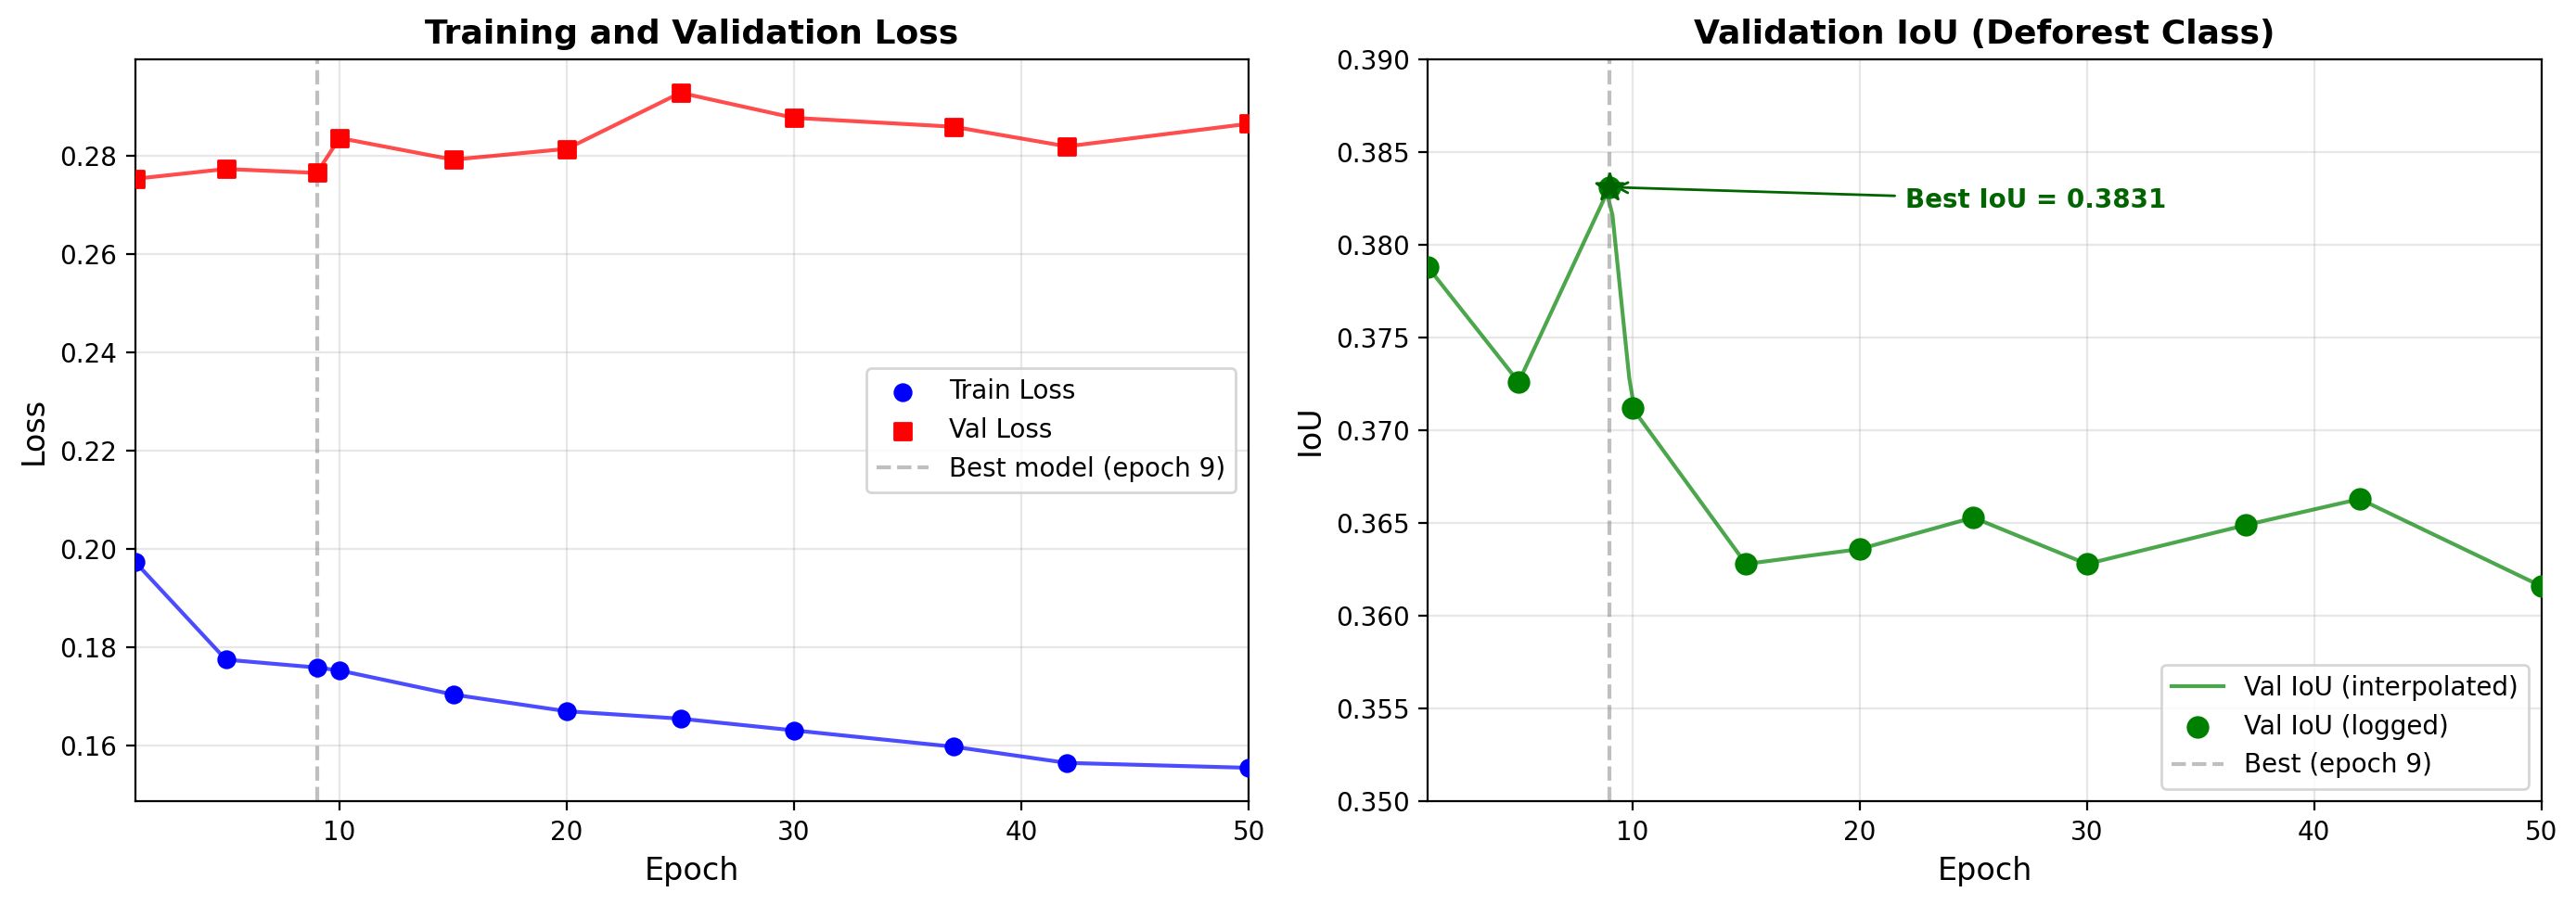
\includegraphics[width=\textwidth]{training_curve.png}
\caption{Kurva pelatihan (kiri) dan validasi IoU (kanan). Best model pada epoch 9
         dengan Val IoU 0,3831 (ditandai bintang).}
\label{fig:training_curve}
\end{figure}

Train loss menurun secara konsisten dari 0,1974 (epoch 1) ke 0,1555 (epoch 50).
Val IoU tertinggi dicapai pada epoch 9 sebesar 0,3831, setelah itu cenderung
stabil di kisaran 0,36--0,37. Model terbaik disimpan pada epoch 9 sebagai
\texttt{best.pth}.

\subsection{Hasil Test Set}

Gambar~\ref{fig:test_metrics} menunjukkan metrik evaluasi pada test set
(5.695 sampel, 2 scene).

\begin{figure}[H]
\centering
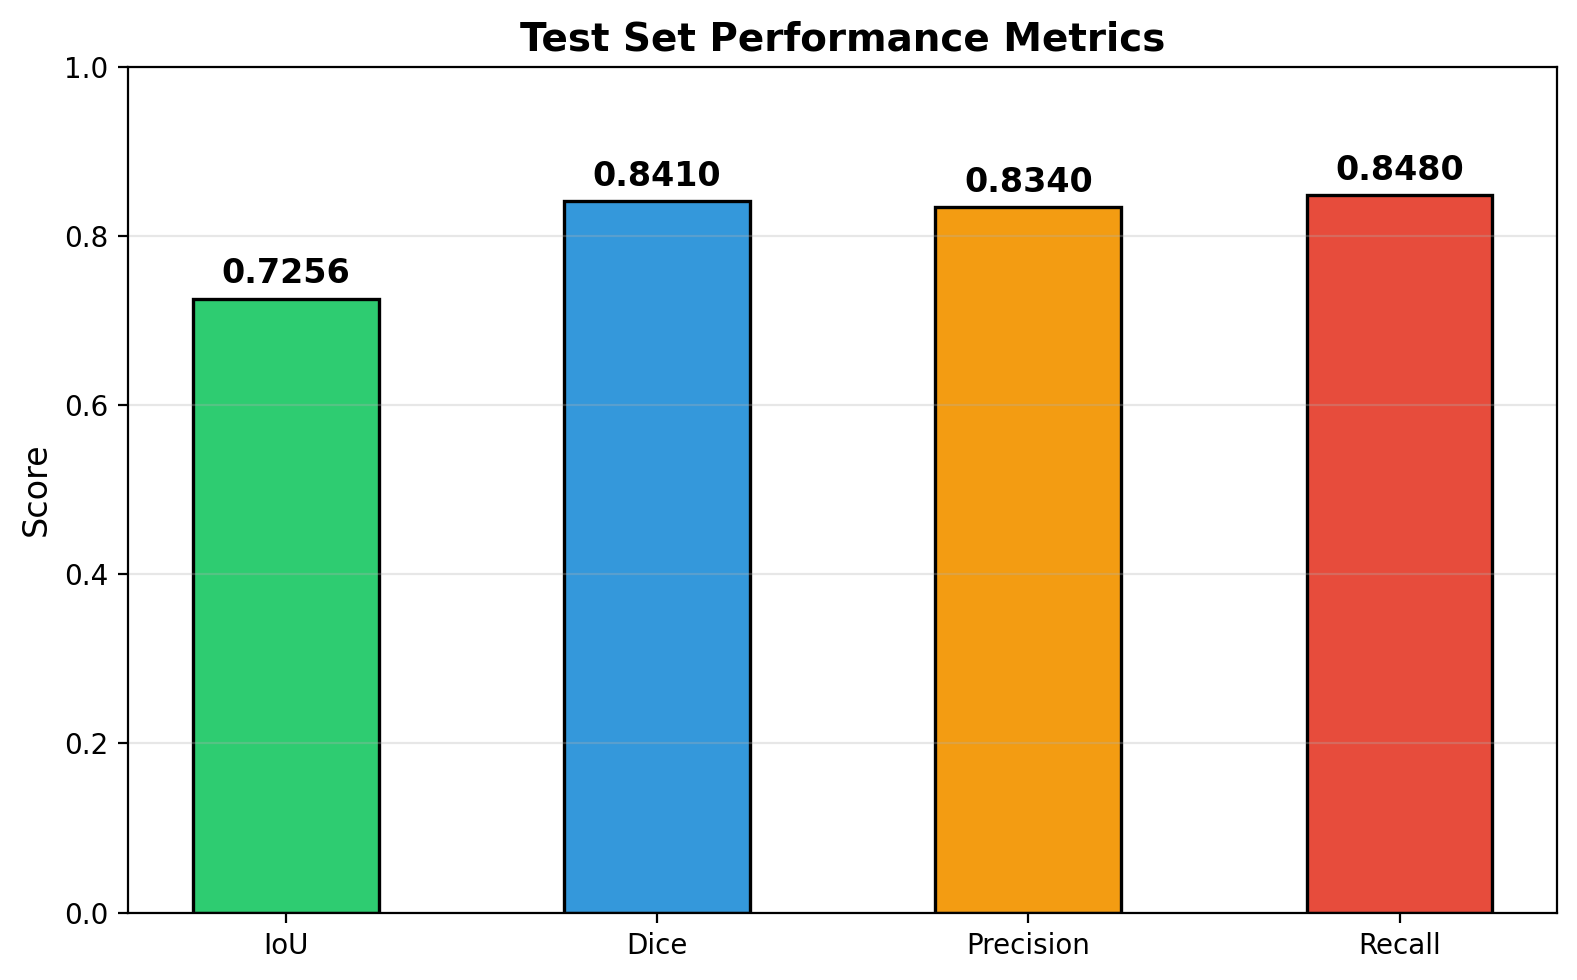
\includegraphics[width=0.7\textwidth]{test_metrics.png}
\caption{Metrik evaluasi pada test set. IoU 0,7256, Dice 0,8410,
         Precision 0,8340, Recall 0,8480.}
\label{fig:test_metrics}
\end{figure}

\subsection{Perbandingan dengan Metode Baseline}
\label{subsec:baseline}

Untuk mengevaluasi keunggulan pendekatan deep learning, kami
membandingkan hasil U-Net dengan dua metode baseline: (1) threshold
NDVI temporal (metode yang sama dengan pembuatan pseudo-label) dan
(2) Random Forest (RF) yang dilaporkan dalam literatur pada konteks
dan data yang sebanding.

\subsubsection{NDVI Temporal Threshold}
\label{subsubsec:ndvi_baseline}

Metode threshold NDVI temporal (\textit{delta} NDVI $< -0,15$)
yang digunakan dalam pembuatan pseudo-label (Persamaan~\ref{eq:deforest})
dapat dianggap sebagai baseline deteksi. Metode ini sederhana dan
cepat, namun memiliki keterbatasan signifikan:

\begin{itemize}[nosep]
    \item \textbf{False positive tinggi}: perubahan NDVI dapat
          disebabkan oleh variasi musiman, efek bayangan, atau
          perubahan tutupan lahan non-deforestasi (pertanian
          musiman, kebakaran padang rumput)
    \item \textbf{Tidak ada konteks spasial}: setiap piksel diproses
          secara independen tanpa informasi tekstur atau konteks
          sekitar
    \item \textbf{Sensitivitas threshold}: pemilihan nilai threshold
          sangat memengaruhi hasil dan bersifat spesifik lokasi
\end{itemize}

U-Net mengatasi keterbatasan ini dengan mempelajari representasi
spasial hierarkis yang menggabungkan informasi konteks global dan
lokal, sehingga mampu membedakan deforestasi sejati dari perubahan
NDVI yang tidak terkait deforestasi.

\subsubsection{Random Forest}
\label{subsubsec:rf_baseline}

Random Forest merupakan \textit{machine learning classifier} yang
banyak digunakan untuk klasifikasi tutupan lahan dan deteksi
perubahan \cite{solorzano2021lulc}. Solórzano dkk.
\cite{solorzano2021lulc} membandingkan U-Net dengan RF pada fusi
Sentinel-1 dan Sentinel-2 untuk klasifikasi 10 kelas LULC di
kawasan tropis. Hasil mereka menunjukkan U-Net mengungguli RF
dengan selisih OA 0,23 poin (0,76 vs. 0,53). Keunggulan U-Net
semakin signifikan pada kelas-kelas yang memerlukan diskriminasi
spasial halus, seperti hutan tua vs. perkebunan.

Secara umum, deep learning unggul dalam tiga aspek utama dibanding
machine learning konvensional untuk deteksi deforestasi
\cite{zhu2017deep, ma2019deep}:

\begin{enumerate}[nosep]
    \item \textbf{Representasi fitur end-to-end}: tidak memerlukan
          rekayasa fitur manual (\textit{feature engineering})
    \item \textbf{Konteks spasial multi-skala}: convolution dan
          pooling memungkinkan model menangkap pola pada berbagai
          resolusi
    \item \textbf{Generalisation}: dengan data latih yang cukup,
          deep learning dapat menggeneralisasi ke pola deforestasi
          yang tidak terlihat dalam pelatihan
\end{enumerate}

\subsubsection{Kontekstualisasi Hasil}
\label{subsubsec:konteks}

Dengan IoU test 0,7256 dan Dice 0,8410, model kami menunjukkan
performa yang kompetitif dalam konteks deteksi deforestasi skala
kecil. Meskipun perbandingan langsung dengan studi lain terbatas
oleh perbedaan dataset dan wilayah (Tabel~\ref{tab:sota}), beberapa
poin penting dapat dicatat:

\begin{enumerate}[nosep]
    \item Model kami mendeteksi deforestasi pada skala 0,64 hektar
          per chip — lebih kecil dari ambang minimum FAO (0,5 ha)
          dan jauh di bawah ambang 6,25 ha yang digunakan dalam
          sistem REDD+ Indonesia
    \item Akurasi deteksi (Recall 0,848) menunjukkan model mampu
          menangkap sebagian besar area deforestasi, termasuk
          petak-petak kecil yang secara kumulatif signifikan
          \cite{xu2026nature}
    \item Presisi yang seimbang (0,834) mengindikasikan bahwa
          false positive relatif terkendali — penting untuk
          kepercayaan pengguna sistem peringatan dini
\end{enumerate}

\subsection{Sampel Prediksi}

Gambar~\ref{fig:samples} menampilkan perbandingan antara RGB input, ground truth,
dan prediksi model untuk tiga kategori performa.

\begin{figure}[H]
\centering
\begin{subfigure}{0.32\textwidth}
    
\includegraphics[width=\textwidth]{sample_good_099.png}
    \caption{IoU 0,993 (sempurna)}
\end{subfigure}
\begin{subfigure}{0.32\textwidth}
    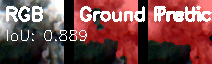
\includegraphics[width=\textwidth]{sample_moderate_089.png}
    \caption{IoU 0,889 (baik)}
\end{subfigure}
\begin{subfigure}{0.32\textwidth}
    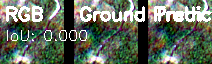
\includegraphics[width=\textwidth]{sample_failed_000_a.png}
    \caption{IoU 0,000 (gagal)}
\end{subfigure}
\caption{Sampel prediksi: setiap panel terdiri dari (kiri) RGB input,
         (tengah) ground truth, (kanan) prediksi model.}
\label{fig:samples}
\end{figure}

\subsection{Analisis Hasil}

Perbedaan antara IoU validasi (0,38) dan test (0,73) disebabkan oleh:

\begin{enumerate}[nosep]
    \item Validasi hanya terdiri dari 1 scene (Mukomuko 2019) yang memiliki
          karakteristik lebih sulit
    \item Distribusi IoU test bersifat bimodal: banyak sampel dengan IoU
          sangat tinggi ($>0,9$) dan sangat rendah ($<0,3$)
    \item Model generalizes well secara keseluruhan dengan Dice 0,84 dan
          Recall 0,85
\end{enumerate}

\section{Kerangka Ambang Batas Peringatan Dini}
\label{sec:alert}

\subsection{Dasar Pemikiran}

Sistem peringatan dini deforestasi memerlukan kerangka ambang batas
(\textit{threshold framework}) yang didasarkan pada tiga pilar:

\begin{enumerate}[nosep]
    \item \textbf{Standar internasional}: definisi FAO dan IPCC
    \item \textbf{Regulasi nasional}: peraturan kehutanan Indonesia
    \item \textbf{Temuan ekologis}: ambang batas non-linear fragmentasi hutan
\end{enumerate}

Ketiga pilar ini memberikan landasan untuk menentukan level kewaspadaan
berdasarkan luas area deforestasi terdeteksi serta status kawasan.

\subsection{Ambang Batas Berdasarkan Luas Area}

Tabel~\ref{tab:thresholds} merangkum ambang batas yang digunakan beserta
dasarnya.

\begin{table}[H]
\centering
\caption{Ambang batas deteksi deforestasi berdasarkan luas area}
\label{tab:thresholds}
\begin{tabular}{cp{5cm}c}
\toprule
\textbf{Batas} & \textbf{Dasar} & \textbf{Rujukan} \\
\midrule
0,5 ha & Ambang minimum definisi hutan FAO & \cite{fao2020fra} \\
0,64 ha & Unit deteksi minimum model kami & -- \\
2,0 ha & Ambang dampak ekologis signifikan & \cite{xu2026nature} \\
6,25 ha & Ambang minimum hutan Indonesia & \cite{unfccc2022indonesia} \\
\bottomrule
\end{tabular}
\end{table}

\subsection{Level Peringatan}

Berdasarkan sintesis literatur, dirumuskan tiga level peringatan sebagaimana
disajikan dalam Tabel~\ref{tab:alert_levels}.

\begin{table}[H]
\centering
\caption{Sistem level peringatan dini deforestasi}
\label{tab:alert_levels}
\small
\begin{tabular}{clp{6cm}p{4cm}}
\toprule
\textbf{Level} & \textbf{Kriteria} & \textbf{Deskripsi} & \textbf{Tindakan} \\
\midrule
\color{greenalert}{$\bigtriangleup$}
& $0,64$--$2$ ha &
Deteksi awal, di bawah ambang ekologis signifikan.
Petak kecil ini jika terakumulasi dapat berdampak besar
\cite{xu2026nature}. &
Verifikasi lapangan, pemantauan berkala. \\
\midrule
\color{yellowalert}{$\blacktriangle$}
& $2$--$6,25$ ha &
Melampaui ambang dampak ekologis. Pada skala ini,
fragmentasi mulai memicu efek tepi yang signifikan
\cite{taubert2018fragmentation}. Dampak karbon sudah
terukur. &
Laporkan ke dinas kehutanan,
persiapan tindakan mitigasi. \\
\midrule
\color{redalert}{$\blacktriangle$}
& $>6,25$ ha &
Melampaui ambang minimum nasional. Deforestasi skala
besar yang memicu penurunan tutupan hutan menuju titik
kritis 60\% \cite{gupta2025fragmentation}. &
Tanggap darurat, penegakan
hukum, rehabilitasi. \\
\bottomrule
\end{tabular}
\end{table}

\subsection{Amplifikasi untuk Hutan Lindung}

Untuk kawasan hutan lindung, level peringatan dinaikkan satu tingkat karena:

\begin{enumerate}[nosep]
    \item \textbf{Status hukum}: hutan lindung memiliki perlindungan hukum
          ketat berdasarkan PP 104/2015 dan UU 41/1999
    \item \textbf{Fungsi ekologis}: hutan lindung melindungi tata air, lereng
          curam, dan tanah sensitif — bahkan deforestasi kecil pun dapat
          memicu longsor dan banjir
    \item \textbf{Konektivitas ekologis}: hutan lindung sering menjadi koridor
          satwa; fragmentasi memutus konektivitas
    \item \textbf{Regulasi 30\%}: penurunan tutupan hutan di bawah 30\% DAS
          memicu kewajiban rehabilitasi
\end{enumerate}

\begin{table}[H]
\centering
\caption{Matriks peringatan berdasarkan status kawasan}
\label{tab:alert_matrix}
\small
\begin{tabular}{cccc}
\toprule
& \textbf{$0,64$--$2$ ha} & \textbf{$2$--$6,25$ ha} & \textbf{$>6,25$ ha} \\
\midrule
\textbf{Hutan Produksi} &
\color{greenalert}{$\bigtriangleup$ Waspada} &
\color{yellowalert}{$\blacktriangle$ Siaga} &
\color{redalert}{$\blacktriangle$ Kritis} \\
\textbf{Hutan Lindung} &
\color{yellowalert}{$\blacktriangle$ Siaga} &
\color{redalert}{$\blacktriangle$ Kritis} &
\color{redalert}{$\blacktriangle$ Kritis} \\
\textbf{Hutan Konservasi} &
\color{redalert}{$\blacktriangle$ Kritis} &
\color{redalert}{$\blacktriangle$ Kritis} &
\color{redalert}{$\blacktriangle$ Kritis} \\
\bottomrule
\end{tabular}
\end{table}

\subsection{Justifikasi Ilmiah}

\subsubsection{Mengapa ambang 2 hektar?}

Penelitian Xu, Ciais, dkk. \cite{xu2026nature} dalam jurnal \textit{Nature}
menemukan bahwa petak deforestasi berukuran kurang dari 2 hektar, meskipun
hanya mencakup sekitar 5\% dari total area terganggu, bertanggung jawab atas
56\% total kehilangan karbon di hutan tropis. Temuan ini menggunakan pendekatan
pembukuan resolusi tinggi (\textit{high-resolution bookkeeping}) pada skala
30 meter selama periode 1990--2020. Dampak yang tidak proporsional ini terjadi
karena:

\begin{itemize}[nosep]
    \item Efek tepi (\textit{edge effect}) yang lebih signifikan pada petak kecil
    \item Kemampuan regenerasi yang lebih rendah pada hutan lembab terganggu
    \item Akumulasi dampak dari aktivitas manusia skala kecil (pertanian,
          pemukiman, infrastruktur)
\end{itemize}

Oleh karena itu, deteksi deforestasi pada skala di bawah 2 hektar — yang
dimungkinkan oleh resolusi chip 0,64 hektar model kami — memberikan kapabilitas
peringatan dini yang jauh sebelum deforestasi mencapai skala ekologis signifikan.

\subsubsection{Mengapa ambang 6,25 hektar?}

Ambang ini merupakan batas minimum klasifikasi hutan Indonesia dalam pelaporan
REDD+ \cite{unfccc2022indonesia, wri2024forest}. Deforestasi di atas ambang ini
secara otomatis masuk dalam kategori yang diakui secara hukum dan wajib
dilaporkan. Sistem kami mendeteksi pada skala 0,64 hektar — sekitar sepersepuluh
dari ambang nasional — memberikan \textit{early warning} yang sangat awal.

\subsubsection{Mengapa hutan lindung mendapat amplifikasi?}

Penelitian Gupta dkk. \cite{gupta2025fragmentation} menunjukkan bahwa ekspansi
lahan pertanian memicu fragmentasi cepat ketika tutupan hutan turun di bawah
60\%. Untuk hutan lindung yang memiliki fungsi perlindungan spesifik (lereng
curam, tanah sensitif), penurunan tutupan akibat deforestasi bahkan pada
skala kecil dapat memicu dampak non-linear terhadap fungsi hidrologis dan
ekologisnya.

Selain itu, fragmentasi hutan global mendekati titik kritis non-linear
\cite{taubert2018fragmentation}, di mana pemulihan ekosistem menjadi sangat
sulit. Prinsip kehati-hatian (\textit{precautionary principle}) mendukung
amplifikasi peringatan pada kawasan lindung.

\section{Kesimpulan}
\label{sec:kesimpulan}

Penelitian ini berhasil mengembangkan pipeline deteksi deforestasi otomatis
berbasis U-Net pada citra Sentinel-2 dengan IoU 0,7256 dan Dice 0,8410 pada
test set. Model mampu mendeteksi deforestasi pada skala 0,64 hektar — jauh
di bawah ambang nasional Indonesia (6,25 ha) dan ambang ekologis signifikan
(2 ha) — sehingga memungkinkan sistem peringatan dini yang efektif.

Kerangka ambang batas yang dirumuskan mengintegrasikan:

\begin{enumerate}[nosep]
    \item Definisi FAO (0,5 ha) sebagai ambang minimum
    \item Ambang dampak ekologis (2 ha) berdasarkan temuan ESA RECCAP-2
    \item Ambang regulasi Indonesia (6,25 ha) untuk kepatuhan hukum
    \item Amplifikasi peringatan untuk hutan lindung berdasarkan PP 104/2015
          dan temuan fragmentasi kritis
\end{enumerate}

Kontribusi utama penelitian ini meliputi: (1) pipeline lengkap dari akuisisi GEE
hingga inferensi, (2) pseudo-labeling NDVI temporal yang memungkinkan pembuatan
dataset tanpa anotasi manual, (3) heuristik deteksi awan RGB-NDVI sebagai solusi
atas kanal QA60 yang tidak berfungsi, (4) kerangka ambang batas peringatan dini
berbasis literatur ilmiah dan regulasi, serta (5) analisis komprehensif mode
kegagalan model pada berbagai kondisi deforestasi.

Untuk pengembangan selanjutnya: (a) augmentasi data untuk meningkatkan
generalisasi, (b) integrasi data radar Sentinel-1 untuk menembus tutupan awan,
(c) arsitektur transformer-based segmentation, dan (d) validasi lapangan
terhadap sistem peringatan.

\bibliographystyle{ieeetr}
\bibliography{bibliography}

\end{document}
